\documentclass[a4paper,oneside,brazil,11pt,a4paper,openright,titlepage,
                usenames,dvipsnames]{book}
% Classe alternativa, apropriada para impressão frente-verso.
% \documentclass[11pt,a4paper,openright,titlepage]{book}

\usepackage[utf8]{inputenc}
\usepackage[T1]{fontenc}
\usepackage[brazilian]{babel}
\usepackage{lmodern}
\usepackage{array}
\usepackage{verbatim}
\usepackage{calc}
\usepackage{textcomp}
\usepackage{gensymb}
\usepackage{amsfonts}
\usepackage{amsmath}
\usepackage[thmmarks,amsmath]{ntheorem}%\usepackage{amsthm}
\usepackage{amssymb}
\usepackage{graphicx}
\usepackage{float}
\usepackage[]{subfigure}
\usepackage{epsfig}
\usepackage{boxedminipage}
\usepackage{geometry}
\usepackage{theorem}
\usepackage{fancybox}
\usepackage{fancyhdr}
\usepackage{ifthen}
\usepackage{afterpage}
\usepackage{color}
\usepackage{colortbl}
\usepackage{rotating}
\usepackage{makeidx}
\usepackage{indentfirst}
\usepackage{import}
\usepackage{enumitem}
\usepackage{pmboxdraw}
\usepackage[hyphens]{url}
\usepackage{hyperref}
\usepackage{longtable}
\usepackage{multirow}
\usepackage{listings}
\lstset{
    frame=tb,
    aboveskip=3mm,
    belowskip=3mm,
    showstringspaces=false,
    basicstyle={\small\ttfamily},
    numbers=none,
    breaklines=true,
    breakatwhitespace=true,
    tabsize=4
}


\usepackage{ft2unb}

\makeindex

\makeatother

\begin{document}
\setcounter{secnumdepth}{4}
\setcounter{tocdepth}{3}
\pagestyle{empty}

\grau{Engenheiro de Controle e Automação}

\tipodemonografia{TRABALHO DE GRADUAÇÃO}

% Título
\titulolinhai{RISC-V SiMPLE:}
\titulolinhaii{Projeto e desenvolvimento de processadores RISC-V}
\titulolinhaiii{com a ISA RV32IMF usando as microarquiteturas}
\titulolinhaiv{Uniciclo, Multiciclo e Pipeline em FPGA}

% Autores
\autori{Arthur de Matos Beggs}
\autorii{}
\autoriii{}

% Membros da banca
\membrodabancai{Prof.\ Marcus Vinicius Lamar, CIC/UnB}
\membrodabancaifuncao{Orientador}

\membrodabancaii{Prof.\ Ricardo Pezzuol Jacobi, CIC/UnB}
\membrodabancaiifuncao{Examinador Interno}


\membrodabancaiii{Prof.\ Marcelo Grandi Mandelli,CIC/UnB}
\membrodabancaiiifuncao{Examinador Interno}

\membrodabancaiv{}
\membrodabancaivfuncao{}

\membrodabancav{}
\membrodabancavfuncao{}

% Data de defesa
\mes{Maio}
\ano{2021}

% Comandos para criar a capa e a página de assinaturas
\capaprincipal{}
\capaassinaturas{}

% Ficha Catalográfica
\noindent \textbf{FICHA CATALOGRÁFICA}

\noindent %
\fbox{\begin{minipage}[t]{1\columnwidth}%
ARTHUR, DE MATOS BEGGS

RISC-V SiMPLE: Projeto e Desenvolvimento de Processadores RISC-V com a ISA RV32IMF
    Usando as Microarquiteturas Uniciclo, Multiciclo e Pipeline em FPGA,

\medskip{}


{[}Distrito Federal{]} 2021.

\medskip{}

% TODO: Número de páginas
viii, 57p., 297 mm (FT/UnB, Engenheiro, Controle e Automação, 2021).
Trabalho de Graduação \textendash{} Universidade de Brasília. Faculdade
de Tecnologia.

\medskip{}


1. RISC-V\hfill{}2. Verilog\hfill{}

3. FPGA

\medskip{}

I. Mecatrônica/FT/UnB\hfill{}

%
\end{minipage}}

\noindent \medskip{}


\noindent \textbf{REFERÊNCIA BIBLIOGRÁFICA}

% TODO: Título final, número de publicação e número de páginas
BEGGS, ARTHUR DE MATOS, (2021). RISC-V SiMPLE: Projeto e Desenvolvimento de
Processadores RISC-V com a ISA RV32IMF Usando as Microarquiteturas Uniciclo,
Multiciclo e Pipeline em FPGA.  Trabalho de Graduação em Engenharia de Controle
e Automação, Publicação FT.TG-$n^{\circ}06$, Faculdade de Tecnologia,
Universidade de Brasília, Brasília, DF, 65p.


\noindent \textbf{CESSÃO DE DIREITOS}

\noindent AUTOR: Arthur de Matos Beggs

\noindent TÍTULO DO TRABALHO DE GRADUAÇÃO: RISC-V SiMPLE: Projeto e Desenvolvimento de
Processadores RISC-V com a ISA RV32IMF Usando as Microarquiteturas Uniciclo,
Multiciclo e Pipeline em FPGA.

\noindent \medskip{}


\noindent GRAU: Engenheiro\hfill{}ANO: 2021\hfill{}

\noindent \medskip{}


É concedida à Universidade de Brasília permissão para reproduzir cópias
deste Trabalho de Graduação e para emprestar ou vender tais cópias
somente para propósitos acadêmicos e científicos. O autor reserva
outros direitos de publicação e nenhuma parte desse Trabalho de Graduação
pode ser reproduzida sem autorização por escrito do autor.

\noindent \bigskip{}


\noindent \rule[0.5ex]{.4\columnwidth}{1pt}

\noindent Arthur de Matos Beggs

\noindent SHCGN 703 Bl G Nº 120, Asa Norte

\noindent 70730-707 Brasília \textendash{} DF \textendash{} Brasil.


% Dedicatória
\frontmatter

\dedicatoriaautori{}
\dedicatoriaautorii{}
\dedicatoriaautoriii{}
\dedicatoria{}

% Agradecimentos
\agradecimentosautori{}
\agradecimentosautorii{}
\agradecimentosautoriii{}
\agradecimentos{}

\resumo{resumo}{
{
    Desenvolvimento e documentação de uma plataforma de ensino de arquitetura
    de computadores em \textit{Verilog} sintetizável em \textit{FPGA}, com foco
    em um processador com arquitetura do conjunto de instruções \textit{RISC-V}
    implementado em três microarquiteturas para ser utilizado como recurso de
    laboratório na disciplina de Organização e Arquitetura de Computadores da
    Universidade de Brasília.
    A plataforma funciona nas \textit{FPGAs terasIC DE1-SoC} disponíveis no
    laboratório da Universidade, possui periféricos de depuração como
    \textit{display} dos registradores do processador na saída de vídeo, além
    de outros periféricos como \textit{drivers} de áudio e vídeo para uma
    experiência mais completa de desenvolvimento, e permite que o processador
    seja substituído por implementações de diversas arquiteturas de
    \textit{32 bits} com certa facilidade.
}

\medskip{}

Palavras Chave: RISC-V, Verilog, FPGA
}\vspace*{2cm}


\resumo{Abstract}{
{
}

\medskip{}

Keywords: RISC-V, Verilog, FPGA
}

% Listas de conteúdo, figuras e tabelas
\sumario{}
\listadefiguras{}
\listadetabelas{}

% Lista de Símbolos
%TCIDATA{LaTeXparent=0,0,these.tex}

\chapter*{LISTA DE SÍMBOLOS}

% \subsection*{Símbolos Latinos}

% \begin{tabular}{p{0.1\textwidth}p{0.63\textwidth}>{\PreserveBacklash\raggedleft}p{0.15\textwidth}}
% $v$  & Velocidade linear  & {[}m/s{]}\tabularnewline
% \end{tabular}


% \subsection*{Símbolos Gregos}

% \begin{tabular}{p{0.1\textwidth}p{0.63\textwidth}>{\PreserveBacklash\raggedleft}p{0.15\textwidth}}
% $\omega$ & Velocidade angular & {[}rad/s{]}\tabularnewline
% \end{tabular}


% \subsection*{Grupos Adimensionais}
%
% \begin{tabular}{p{0.1\textwidth}p{0.8\textwidth}}
% i, k & Contador\tabularnewline
% \end{tabular}


% \subsection*{Subscritos}

% \begin{tabular}{p{0.1\textwidth}p{0.8\textwidth}}
% $ref$  & referência \tabularnewline
% $fer$  & ferramenta \tabularnewline
% $sis$  & sistema \tabularnewline
% $des$  & desejado\tabularnewline
% \end{tabular}


% \subsection*{Sobrescritos}

% \begin{tabular}{p{0.1\textwidth}p{0.8\textwidth}}
% $\cdot$  & Variação temporal \tabularnewline
% $-$  & Valor médio \tabularnewline
% \end{tabular}


\subsection*{Siglas}

\begin{tabular}{p{0.1\textwidth}p{0.8\textwidth}}
    {ASIC}      & {Circuito Integrado de Aplicação Específica --- \textit{Application Specific Integrated Circuit}}\tabularnewline{}
    {AWS}       & {\textit{Amazon Web Services}} \tabularnewline{}
    {BSD}       & {Distribuição de Software de Berkeley --- \textit{Berkeley Software Distribution}}\tabularnewline{}
    {CISC}      & {Computador com Conjunto de Instruções Complexo --- \textit{Complex Instruction Set Computer}} \tabularnewline{}
    {CSR}       & {Registradores de Controle e Estado --- \textit{Control and Status Registers}} \tabularnewline{}
    {DSP}       & {Processamento Digital de Sinais --- \textit{Digital Signal Processing}} \tabularnewline{}
    {FPGA}      & {Arranjo de Portas Programáveis em Campo --- \textit{Field Programmable Gate Array}} \tabularnewline{}
    {hart}      & {\textit{hardware thread}} \tabularnewline{}
    {ISA}       & {Arquitetura do Conjunto de Instruções --- \textit{Instruction Set Architecture}} \tabularnewline{}
    {MIPS}      & {Microprocessador sem Estágios Intertravados de \textit{Pipeline} --- \textit{Microprocessor without Interlocked Pipeline Stages}} \tabularnewline{}
    {OAC}       & {Organização e Arquitetura de Computadores} \tabularnewline{}
    {PC}        & {Contador de Programa --- \textit{Program Counter}} \tabularnewline{}
    {PLL}       & {Malha de Captura de Fase --- \textit{Phase-Locked Loop}} \tabularnewline{}
    {RAS}       & {Pilha de Endereços de Retorno --- \textit{Return Address Stack}} \tabularnewline{}
    {RISC}      & {Computador com Conjunto de Instruções Reduzido --- \textit{Reduced Instruction Set Computer}} \tabularnewline{}
    {SBC}       & {Computadores em Placa Única --- \textit{Single Board Computers}} \tabularnewline{}
    {SDK}       & {Conjunto de Programas de Desenvolvimento --- \textit{Software Development Kit}} \tabularnewline{}
    {SiMPLE}    & {Ambiente de Aprendizado Uniciclo, Multiciclo e \textit{Pipeline} --- \textit{Single-cycle Multicycle Pipeline Learning Environment}} \tabularnewline{}
    {SoC}       & {Sistema em um Chip --- \textit{System on Chip}} \tabularnewline{}
    {TSMC}      & {\textit{Taiwan Semiconductor Manufacturing Company}} \tabularnewline{}
     % &  \tabularnewline
     % &  \tabularnewline
     % &  \tabularnewline
\end{tabular}


% Corpo Principal
\mainmatter{}
\setcounter{page}{1}
\pagenumbering{arabic}
\pagestyle{plain}

%% Template de imagem
% \begin{figure}[H]
% \centering
% \includegraphics[width=.7\linewidth]
%     {../images/}
%     \caption[]
%         {}\label{fig:}
% \end{figure}

\chapter{Introdução}\label{cap_intro}

%\resumodocapitulo{Resumo opcional}

\section{Motivação}
{
    O mercado de trabalho está a cada dia mais exigente, sempre buscando
    profissionais que conheçam as melhores e mais recentes ferramentas
    disponíveis. Além disso, muitos universitários se sentem desestimulados
    ao estudarem assuntos desatualizados e com baixa possibilidade de
    aproveitamento do conteúdo no mercado de trabalho. Isso alimenta o
    desinteresse pelos temas abordados e, em muitos casos, leva à evasão
    escolar. Assim, é importante renovar as matérias com novas tecnologias
    e tendências de mercado sempre que possível, a fim de instigar o
    interesse dos discentes e formar profissionais mais capacitados e
    preparados para as demandas da atualidade.
}

{
    Até recentemente, a disciplina de Organização e Arquitetura de Computadores
    da Universidade de Brasília era ministrada em todas as turmas utilizando a
    arquitetura \textit{MIPS32}. Apesar da arquitetura \textit{MIPS32} ainda ter
    grande força no meio acadêmico (em boa parte devido a sua simplicidade e
    extensa bibliografia), sua aplicação na indústria tem diminuído
    consideravelmente na última década.
}

{
    Embora a curva de aprendizagem de linguagens \textit{assembly} de alguns
    processadores \textit{RISC} seja relativamente baixa para quem já conhece o
    \textit{assembly MIPS32}, aprender uma arquitetura atual traz o benefício de
    conhecer o \textit{estado da arte} da organização e arquitetura de
    computadores.
}

{
    Hoje, a disciplina também é ministrada na arquitetura \textit{ARM}, bem como
    na \textit{ISA RISC-V}, desenvolvida na Divisão de Ciência da Computação da
    Universidade da Califórnia - Berkeley, e será o objeto de estudo desse
    trabalho.
}


\section{Por que RISC-V?}
{
    A \textit{ISA RISC-V} (lê-se \textit{``risk-five''}) é uma arquitetura
    \textit{open source}~\cite{riscv_spec} com licença \textit{BSD}, o que
    permite o seu livre uso para quaisquer fins, sem distinção de se o trabalho
    possui código-fonte aberto ou proprietário. Tal característica possibilita
    que grandes fabricantes utilizem a arquitetura para criar seus produtos,
    mantendo a proteção de propriedade intelectual sobre seus métodos de
    implementação e quaisquer subconjuntos de instruções não-\textit{standard}
    que as empresas venham a produzir, o que estimula investimentos em pesquisa
    e desenvolvimento.
}

{
    Empresas como Google, IBM, Nvidia, Samsung, Qualcomm e Western Digital são
    algumas das fundadoras e investidoras da \textit{RISC-V Foundation}, órgão
    responsável pela governança da arquitetura. Isso demonstra o interesse das
    gigantes do mercado no sucesso e disseminação da arquitetura.
}

{
    A licença também permite que qualquer indivíduo produza, distribua e
    até mesmo comercialize sua própria implementação da arquitetura sem ter
    que arcar com \textit{royalties}, sendo ideal para pesquisas acadêmicas,
    \textit{startups} e até mesmo \textit{hobbyistas}.
}

{
    O conjunto de instruções foi desenvolvido tendo em mente seu uso em
    diversas escalas: sistemas embarcados, \textit{smartphones},
    computadores pessoais, servidores e supercomputadores, o que permitirá
    maior reuso de \textit{software} e maior integração de
    \textit{hardware}.
}

{
    Outro fator que estimula o uso do \textit{RISC-V} é a modernização dos
    livros didáticos. A nova versão do livro utilizado em OAC, Organização
    e Projeto de Computadores, de David Patterson e John Hennessy, utiliza
    a \textit{ISA RISC-V}.
}

{
    Além disso, com a promessa de se tornar uma das arquiteturas mais utilizadas
    nos próximos anos, utilizar o \textit{RISC-V} como arquitetura da disciplina
    de OAC se mostra a escolha ideal no momento.
}

\section{O Projeto RISC-V SiMPLE}
{
    O projeto \textit{RISC-V SiMPLE (Single-cycle Multicycle Pipeline Learning
    Environment)} consiste no aprimoramento e documentação do processador com
    conjunto de instruções \textit{RISC-V}, sintetizável em \textit{FPGA} e com
    \textit{hardware} descrito em \textit{Verilog} utilizado como material de
    laboratório de uma das turmas da disciplina de OAC. O objetivo é ter uma
    plataforma de testes e simulação bem documentada e com o mínimo de
    \textit{bugs} para servir de referência na disciplina. O projeto implementa
    três microarquiteturas que podem ser escolhidas a tempo de síntese:
    uniciclo, multiciclo e \textit{pipeline}, todas as três com um \textit{hart}
    e caminho de dados de 32 bits.

    Os processadores contém o conjunto de instruções I (para operações com
    inteiros, sendo o único módulo com implementação mandatória pela
    arquitetura) e as extensões \textit{standard} M (para multiplicação e
    divisão de inteiros) e F (para ponto flutuante com precisão simples conforme
    o padrão IEEE 754 com revisão de 2008). O projeto não implementa as
    extensões D (ponto flutuante de precisão dupla) e A (operações atômicas de
    sincronização), e com isso o \textit{soft core} desenvolvido não pode ser
    definido como de propósito geral, G (que deve conter os módulos I, M, A, F
    e D). Assim, pela nomenclatura da arquitetura, os processadores
    desenvolvidos são do tipo \textit{RV32IMF}.

    O projeto também contempla \textit{traps}, interrupções, exceções,
    \textit{CSRs}, chamadas de sistema e outras funcionalidades de nível
    privilegiado da arquitetura~\cite{riscv_spec2}.
}


\chapter{Revisão Teórica}\label{cap_revisao}
{ Alguns conceitos são essenciais para compreender o projeto proposto, sua
    implementação e seus resultados. Esse capítulo abordará o que é arquitetura
    e organização de computadores, tratará brevemente sobre as arquiteturas mais
    conhecidas e se aprofundará na especificação da arquitetura \textit{RISC-V}.
    Além disso, serão expostos os conceitos de síntese de \textit{hardware} e
    do funcionamento das \textit{FPGAs}, em especial o modelo que será utilizado
    para desenvolver o trabalho.
    Por fim, o ``estado da arte'' da arquitetura \textit{RISC-V} será discutido.
}

\section{Arquitetura de Computadores}
{ Para nos comunicarmos, necessitamos de uma linguagem, e no caso dos
    brasileiros, essa linguagem é o português. Como toda linguagem, o português
    possui sua gramática e dicionário que lhe dá estrutura e sentido. Línguas
    humanas como o português, inglês e espanhol são chamadas de linguagens
    naturais, e evoluíram naturalmente a partir do uso e
    repetição.~\cite{lyons1991natural}
}

{ Por causa da excelente capacidade de interpretação e adaptação da mente
    humana, somos capazes de criar e entender novos dialetos que não seguem as
    regras formais das linguagens naturais que conhecemos. Porém, fora da
    comunicação casual é importante e às vezes obrigatório que nos expressemos
    sem ambiguidade. Línguas artificiais como a notação matemática e linguagens
    de programação possuem semântica e sintaxe mais rígidas para garantir que
    a mensagem transmitida seja interpretada da maneira correta. Sem essa
    rigidez, os computadores de hoje não seriam capazes de entender nossos
    comandos.
}

{ Para a comunicação com o processador de um computador, utilizamos mensagens
    chamadas de instruções, e o conjunto dessas instruções é chamado de
    Arquitetura do Conjunto de Instruções (\textit{ISA}). Um processador só é
    capaz de entender as mensagens que obedecem as regras semânticas e
    sintáticas de sua \textit{ISA}, e qualquer instrução que fuja das suas
    regras causará um erro de execução ou realizará uma tarefa diferente da
    pretendida. A linguagem de máquina é considerada de baixo nível pois
    apresenta pouca ou nenhuma abstração em relação à arquitetura.
}

{ As instruções são passadas para o processador na forma de código de máquina,
    sequências de dígitos binários que correspondem aos níveis lógicos do
    circuito. Para melhorar o entendimento do código e facilitar o
    desenvolvimento, uma outra representação é utilizada, o \textit{assembly}.
    Um código \textit{assembly} é transformado em código de máquina por um
    programa montador, (\textit{assembler}), e o processo inverso é realizado
    por um \textit{disassembler}. As linguagens \textit{assembly}, dependendo do
    \textit{assembler} utilizado, permitem o uso de macros de substituição e
    pseudo instruções (determinadas instruções que não existem na \textit{ISA}
    que são expandidas em instruções válidas pelo montador) e são totalmente
    dependentes da arquitetura do processador, o que normalmente impede que o
    mesmo código seja executado em arquiteturas diferentes.
}

{ A Figura~\ref{fig:cpu_abstraction} é uma representação simplificada de um
    processador. A unidade de controle lê uma instrução da memória e a
    decodifica; o circuito de lógica combinacional lê os dados dos
    registradores, entrada e memória conforme necessário, executa a instrução
    decodificada e escreve no banco de registradores, na memória de dados ou
    na saída se for preciso; a unidade de controle lê uma nova instrução e o
    ciclo se repete até o fim do programa. A posição de memória da instrução
    que está sendo executada fica armazenada em um registrador especial chamado
    de Contador de Programa (\textit{PC}). Algumas instruções modificam o
    \textit{PC} condicionalmente ou diretamente, criando a estrutura para
    saltos, laços e chamada/retorno de funções.
}

\begin{figure}[H]
\centering
\includegraphics[width=.7\linewidth]
    {../images/ABasicComputer.png}
    \caption[Abstração da arquitetura de um computador]
    {Abstração da arquitetura de um
        computador. Fonte:~\cite{wikimedia2015basiccpu}}\label{fig:cpu_abstraction}
\end{figure}

{ Historicamente, as arquiteturas são divididas em \textit{ISAs}
    \textit{RISC} e \textit{CISC}. Na atualidade, a diferença entre elas é que
    as \textit{ISAs RISC} acessam a memória por instruções de
    \textit{load/store}, enquanto as \textit{CISC} podem acessar a memória
    diretamente em uma instrução de operação lógica ou aritmética.
}

{ Algumas arquiteturas \textit{RISC} notáveis são a \textit{RISC-V}, objeto de
    estudo desse trabalho, a \textit{ARM} e a \textit{MIPS}. Quanto às
    \textit{CISC}, a \textit{x86} e sua extensão de 64 \textit{bits}, a
    \textit{AMD64}, são as mais conhecidas.
}

    \subsection{Arquitetura MIPS}
    {}

    \subsection{Arquitetura ARM}
    {}

    \subsection{Arquitetura x86}
    {}

    \subsection{Arquitetura AMD64}
    {}

    \subsection{Arquitetura RISC-V}
    { A \textit{ISA RISC-V} é uma arquitetura modular, sendo o módulo base de
        operações com inteiros mandatório em qualquer implementação. Os demais
        módulos são extensões de uso opcional. A arquitetura não suporta
        \textit{branch delay slots} e aceita instruções de tamanho variável. A
        codificação das instruções de tamanho variável é mostrada na
        Figura~\ref{fig:riscv_var_length}. As instruções presentes no módulo
        base correspondem ao mínimo necessário para emular por
        \textit{software} as demais extensões (com exceção das operações
        atômicas).
    }

    \begin{figure}[H]
    \centering
        \includegraphics[width=1\linewidth]{../images/RV_InstructionLength.png}
        \caption{Codificação de instruções de tamanho variável da arquitetura
                    \textit{RISC-V}}\label{fig:riscv_var_length}
    \end{figure}

    { A nomenclatura do conjunto de instruções implementado segue a
        seguinte estrutura:
    }

    \begin{itemize}[leftmargin=20mm]
        \item {As letras ``RV'';}
        \item {A largura dos registradores do módulo Inteiro;}
        \item {A letra ``I'' representando a base Inteira. Caso o subconjunto
                Embarcado (\textit{Embedded}) seja implementado, substitui-se
                pela letra ``E'';}
        \item {Demais letras identificadoras de módulos opcionais.}
    \end{itemize}

    { Assim, uma implementação com registradores de 32 bits somente com o
        módulo base de Inteiros é denominado ``RV32I''.
    }

        \subsubsection{Módulo Inteiro}
        { O módulo Inteiro é o módulo base da arquiterura. O \textit{design} de sua
            especificação visa reduzir o \textit{hardware} necesário para uma
            implementação mínima, bem como ser um alvo de compilação satisfatório.
        }

        { Diferente de outras arquiteturas como a \textit{ARM}, as instruções de
            multiplicação e divisão não fazem parte do conjunto básico uam vez que
            necessitam de circuito especializado e por isso encarecem o desenvolvimento
            e produção dos processadores.
        }

        { Para sistemas embarcados com restrições mais severas de tamanho, custo,
            potência, etc o módulo base I pode ser substituído por um \textit{subset},
            o módulo E. Porém, nenhuma das demais extensões pode ser usada em conjunto
            com o módulo E.
        }

        \subsubsection{Extensões}
            \paragraph{Extensão M}
            { A extensão M implementa as operações de multiplicação e divisão de
                números inteiros.
            }

            \paragraph{Extensão A}
            { A extensão A implementa instruções de acesso atômico a memória.
                Instruções atômicas mantém a coerência da memória em sistemas
                preemptivos e paralelos.
            }

            \paragraph{Extensão F}
            { A extensão F implementa as isntruções de ponto flutuante IEEE 754 de
                precisão simples, bem como o banco de registradores especializado para
                operações com ponto flutuante.
            }

            \paragraph{Extensão D}
            { A extensão D implementa as instruções de ponto flutuante IEEE 754 de
                precisão dupla. Ela é um incremento à extensão F, sendo esta de
                implementação obrigatória para se poder implementar a extensão D.
            }

            \paragraph{Outras Extensões}
            { Outras extensões são previstas na especificação da arquitetura, e.g.
                a extensão C para instruções comprimidas (16 bits).
            }

            { A arquitetura prevê a expansão de extensões, com alguns
                \textit{opcodes} sendo reservados para essa finalidade. Desse modo,
                instruções proprietárias e/ou customisadas podem ser adicionadas.
            }

        \subsubsection{Arquitetura Privilegiada}
        { Para a \textit{ISA RISC-V}, existem quatro níveis de privilégio de acesso,
            sendo eles o de usuário (módulo I e extensões), de máquina
            (\textit{syscalls}) de supervisor (sistema operacional) e hipervisor
            (virtualização).
        }

        \subsubsection{Formatos de Instruções}
        { As instruções da arquitetura podem ser separadas em subgrupos de acordo com
            os operadores necessários para o processador interpretá-la. A
            Figura~\ref{fig:riscv_formats} apresenta os formatos das instruções do
            módulo I da \textit{ISA RISC-V}, e, para efeitos de comparação, a
            Figura~\ref{fig:mips_formats} mostra os formatos de instruções equivalentes
            na arquitetura MIPS32.
        }

        \begin{figure}[H]
        \centering
            \includegraphics[width=1\linewidth]{../images/RV_Formats.png}
            \caption{Formatos de Instruções da \textit{ISA RISC-V}
                }\label{fig:riscv_formats}
        \end{figure}

        \begin{figure}[H]
        \centering
            \includegraphics[width=1\linewidth]{../images/MIPS_Formats.png}
            \caption{Formatos de Instruções da \textit{ISA MIPS32}
                }\label{fig:mips_formats}
        \end{figure}

        \subsubsection{Formatos de Imediatos}
        { Os imediatos são operandos descritos na própria instrução em vez de estar
            contido em um registrador. Como os operandos necessitam ter a mesma largura
            que o banco de registradores, algumas regras são utilizadas para gerar os
            operandos imediatos. As figuras a seguir mostram a formação de cada tipo de
            imediato dos formatos da Figura~\ref{fig:riscv_formats}.
        }

        \begin{figure}[H]
        \centering
            \includegraphics[width=1\linewidth]{../images/RV_I_Imm.png}
            \caption{Formação do Imediato de tipo I
                }\label{fig:riscv_i_imm}
        \end{figure}

        \begin{figure}[H]
        \centering
            \includegraphics[width=1\linewidth]{../images/RV_S_Imm.png}
            \caption{Formação do Imediato de tipo S
                }\label{fig:riscv_s_imm}
        \end{figure}

        \begin{figure}[H]
        \centering
            \includegraphics[width=1\linewidth]{../images/RV_B_Imm.png}
            \caption{Formação do Imediato de tipo B
                }\label{fig:riscv_b_imm}
        \end{figure}

        \begin{figure}[H]
        \centering
            \includegraphics[width=1\linewidth]{../images/RV_U_Imm.png}
            \caption{Formação do Imediato de tipo U
                }\label{fig:riscv_u_imm}
        \end{figure}

        \begin{figure}[H]
        \centering
            \includegraphics[width=1\linewidth]{../images/RV_J_Imm.png}
            \caption{Formação do Imediato de tipo J
                }\label{fig:riscv_j_imm}
        \end{figure}

        { Para efeitos comparativos, a Figura~\ref{fig:mips_immediates} mostra a
            formação de imediatos na arquitetura MIPS32.
        }

        \begin{figure}[H]
        \centering
            \includegraphics[width=1\linewidth]{../images/MIPS_Immediates.png}
            \caption{Formatos de Imediato da \textit{ISA MIPS32}}\label{fig:mips_immediates}
        \end{figure}


\section{Microarquiteturas}
{}

    \subsection{Uniciclo}
    {}

    \subsection{Multiciclo}
    {}

    \subsection{Pipeline}
    {}

\section{Representação de Hardware}
{}

    \subsection{VHDL}
    {}

    \subsection{Verilog}
    {}

\section{Síntese Lógica}
{}

    \subsection{Análise e Síntese}
    {}

    \subsection{Fitting}
    {}

    \subsection{Timing Analyzer}
    {}

\section{Field Programmable Gate Arrays}
{ \textit{Field Programmable Gate Arrays} (\textit{FPGAs}) são circuitos
    integrados que permitem o desenvolvimento de circuitos lógicos
    reconfiguráveis. Por serem reprogramáveis, as \textit{FPGAs} geram uma
    grande economia em tempo de desenvolvimento e em custos como os de
    prototipagem, validação e manufatura do projeto em relação aos circuitos de
    aplicações específicas, os \textit{ASICs}, e aos projetos
    \textit{full-custom}. As \textit{FPGAs} podem ser tanto o passo
    intermediário no projeto de um \textit{ASIC} ou \textit{full-custom} quanto
    o meio final do projeto quando a reconfigurabilidade e os preços muito mais
    acessíveis forem fatores importantes.
}

{ Cada fabricante de \textit{FPGAs} possui seus \textit{softwares} de
    desenvolvimento, ou \textit{SDKs}. A indústria de \textit{hardware} é
    extremamente protecionista com sua propriedade intelectual, sendo a maioria
    dessas ferramentas de código proprietário. Para a Intel Altera®, essa
    plataforma é o Quartus Prime®.
}

{ \textit{FPGAs} mais modernas possuem, além do arranjo de portas lógicas,
    blocos de memória, \textit{PLLs}, \textit{DSPs} e \textit{SoCs}. Os blocos
    de memória internos funcionam como a memória \textit{cache} de um
    microprocessador, armazenando os dados próximo ao seu local de
    processamento para diminuir a latência. Os \textit{PLLs} permitem criar
    sinais de \textit{clock} com diversas frequências a partir de um relógio de
    referência, e podem ser reconfigurados a tempo de execução. \textit{DSPs}
    são responsáveis pelo processamento de sinais analógicos discretizados, e
    podem ser utilizados como multiplicadores de baixa latência. Já os
    \textit{SoCs} são microprocessadores como os ARM® presentes em celulares,
    e são capazes de executar sistemas operacionais como o Linux.
}

{ Além de disponíveis na forma de \textit{chips} para a integração com placas
    de circuito impresso customizadas, as \textit{FPGAs} possuem \textit{kits}
    de desenvolvimento com diversos periféricos para auxiliar no processo de
    criação de soluções. Esses \textit{kits} são a principal ferramenta de
    aprendizagem no universo dos circuitos reconfiguráveis. No Laboratório de
    Informática da UnB, as placas \textit{terasIC DE1-SoC} com a \textit{FPGA
    Intel® Cyclone V SoC} estão disponíveis para os alunos de OAC desenvolverem
    seus projetos.
}

    \subsection{Arquitetura Generalizada de uma FPGA}
    { De forma genérica, uma \textit{FPGA} possui blocos lógicos, chaves de
        interconexão, blocos de conexão direta e portas de entrada e saída,
        conforme apresentado na Figura~\ref{fig:fpga_general_arch}.
    }

    \begin{figure}[H]
    \centering
    \includegraphics[width=.7\linewidth]
        {../images/fpga_architecture_abstraction_-_olin_college.jpg}
        \caption[Abstração da arquitetura de uma FPGA]
            {Abstração da arquitetura de uma FPGA.\quad Fonte:~\cite{fpga_arch_abstraction}}
        \label{fig:fpga_general_arch}
    \end{figure}

    { Os blocos lógicos possuem \textit{lookup tables}, registradores, somadores
        e multiplexadores. É neles que a lógica reconfigurável é implementada.
    }

    { Já as chaves de interconexão são responsáveis por conectar os diversos
        blocos da \textit{FPGA}. A Figura~\ref{fig:fpga_switch_box} exemplifica
        como é feito o roteamento da malha de interconexão. Os blocos de conexão
        direta são um tipo especial de chave de interconexão, e sua função é ligar
        blocos lógicos adjacentes.
    }

    { Por fim, as portas de entrada e saída conectam a \textit{FPGA} ao ``mundo
        externo'' e.g. \textit{drivers} de áudio e vídeo.
    }

    \begin{figure}[H]
    \centering
    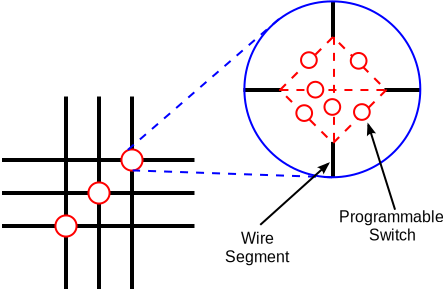
\includegraphics[width=.5\linewidth]
        {../images/switch_box_wikimedia.png}
        \caption[Funcionamento da chave de interconexão]
            {Funcionamento da chave de interconexão.\quad Fonte:~\cite{fpga_switch_box}}
        \label{fig:fpga_switch_box}
    \end{figure}


    \subsection{Arquitetura da FPGA Cyclone V SoC}
    { A Figura~\ref{fig:cyclone_v_arch} apresenta a arquitetura da
        \textit{FPGA Cyclone V SoC}. O \textit{chip} possui um processador
        \textit{ARM} integrado, blocos de memória embutidos, \textit{DSPs} para
        acelerar operações como multiplicação de números ou processamento de
        sinais genéricos, diversos pinos para integrar o \textit{chip} a
        um projeto de circuito mais complexo, \textit{PLLs} para gerar diversos
        sinais de \textit{clock}, entre outras funcionalidades.
    }

    \begin{figure}[H]
    \centering
    \includegraphics[width=1\linewidth]
        {../images/altera_cyclone_v_soc_architectural_downscale.jpg}
        \caption[Arquitetura da FPGA Intel Cyclone V SoC]
            {Arquitetura da \textit{FPGA Altera Cyclone V SoC}.\quad Fonte:~\cite{cyclone_v_soc}}
        \label{fig:cyclone_v_arch}
    \end{figure}

        \subsubsection{Adaptative Logic Modules}
        { Os blocos lógicos, como mostrados na abstração da Figura~\ref{fig:fpga_general_arch}
            são implementados na \textit{FPGA Cyclone V SoC} como
            \textit{Adaptative Logic Modules}, conforme a Figura~\ref{fig:fpga_alm}.
            Como os \textit{ALMs} são blocos genéricos, há um \textit{trade-off}
            entre configurabilidade e performance.
        }

        \begin{figure}[H]
        \centering
        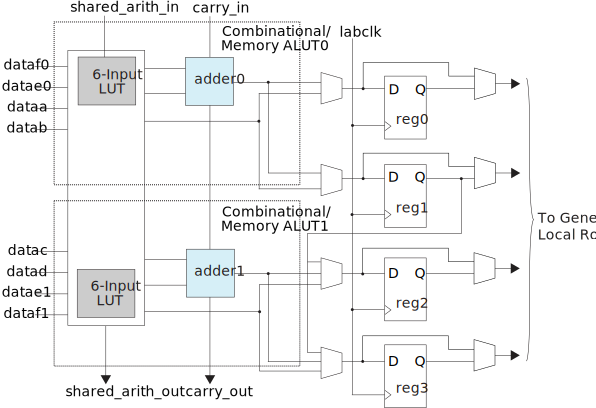
\includegraphics[width=.8\linewidth]
            {../images/intel_alm_high_level.png}
            \caption[Diagrama de blocos de um ALM]
                {Diagrama de blocos de um ALM.\quad Fonte:~\cite{cyclone_alm}}
            \label{fig:fpga_alm}
        \end{figure}


        \subsubsection{Embedded Memory Blocks}
        { Como mostrado na Figura~\ref{fig:cyclone_v_arch}, existem blocos de
            memória embutidos na \textit{FPGA}. Esses blocos são o equivalente
            a uma memória \textit{cache L1}, sendo a camada de memória mais próxima
            dos registradores. Para utilizá-los no \textit{design} do circuito,
            blocos do \textit{IP} de memória são configurados e instanciados
            pelo programa de desenvolvimento para gerar um módulo integrável no
            resto do \textit{design}.
        }

        { As placas de desenvolvimento podem possuir outros tipos de memória,
            como as \textit{SRAM} e \textit{DRAM}. Apesar de possuírem capacidade
            de armazenamento bem maiores que os blocos embutidos, seus
            módulos controladores são mais complexos e apresentam latência maior
            para leitura e escrita de dados. Para seu uso eficiente, é necessário
            implementar camadas de \textit{caching} para que as operações de
            \textit{input} e \textit{output} (\textit{IO}) não se tornem um
            gargalo que comprometa o resto do \textit{design}.
        }


\section{Estado da Arte dos processadores RISC-V}
{ Por alguns anos, processadores com arquitetura \textit{RISC-V} só podiam
    ser utilizados por meio de emuladores como o \textit{qemu}~\cite{qemu_riscv}
    ou em \textit{FPGAs}, o objeto desse trabalho. Algumas fabricantes já
    divulgaram planos para começar a usar microcontroladores com a arquitetura
    em seus produtos, como é o caso dos controladores de discos rígidos e
    \textit{SSDs} da \textit{Western Digital}~\cite{western_riscv} e da Nvidia
    como o substituto dos controladores \textit{Falcon} de suas placas de
    vídeo~\cite{nvidia_riscv}.  Porém, ainda não se sabe se as empresas já
    utilizam os controladores em seus \textit{hardwares}, se a adoção ainda
    está em fase de projeto ou se a ideia foi abandonada.
}

{ Porém, começam a surgir no mercado microcontroladores e \textit{Single
    Board Computers (SBCs)} com preços acessíveis. Placas como a linha
    \textit{Sipeed} da \textit{Seed} se equiparam aos \textit{MCUs
    ESP32}~\cite{hackaday_sipeed}, e outras como a \textit{SiFive HiFive1}
    se assemelham aos \textit{arduinos}~\cite{hifive_arduino}.
    Também é possível utilizar processadores de alto desempenho como o
    \textit{BOOM} em instâncias \textit{EC2 F1} da \textit{AWS}~\cite{boom_aws}.
}

{ Há uma expectativa de \textit{SBCs} mais robustos, capazes de rodar um
    sistema operacional de uso geral, como um \textit{Raspberry Pi}. Existem
    alguns pré-lançamentos de placas para atender essa demanda, como a
    \textit{SiFive HiFive Unmatched}~\cite{hifive_unmatched} e a
    \textit{BeagleV}~\cite{beaglev}.
}

{ A empresa \textit{SiFive}, liderada pelos criadores da arquitetura, produzirá
    em parceria com a \textit{TSMC (Taiwan Semiconductor Manufacturing Company)}
    o primeiro processador \textit{RISC-V} de 32 \textit{bits} em tecnologia
    de 5nm~\cite{sifive_tsmc}. A \textit{TSMC} é a \textit{foundry} líder em
    manufatura de circuitos integrados no mundo.
}

{ Atualmente, compilar códigos em \textit{C/C++} para \textit{targets RISC-V}
    não envolve mais a instalação de \textit{toolchains} complicadas e frágeis.
    Tanto o \textit{gcc}~\cite{gcc_riscv} quanto o \textit{clang}~\cite{clang_riscv}
    já oferecem suporte para o \textit{RISC-V}, eliminando assim uma barreira
    para a adoção da arquitetura.
}

{ Uma outra característica essencial para o uso do \textit{RISC-V} em sistemas
    de uso geral é a existência de sistemas operacionais que funcionem na
    plataforma. Desde a versão 4.15, o \textit{kernel} do \textit{linux}
    oferece suporte para a arquitetura~\cite{linux_kernel}. \textit{Distros}
    como \textit{Fedora}~\cite{fedora_experimental},
    e \textit{Alpine}~\cite{alpine_experimental} já possuem suporte experimental.
    A chinesa \textit{Alibaba} fez o \textit{port} do \textit{OS Android}
    para um de seus \textit{SoCs RISC-V}~\cite{alibaba_android}. Alguns
    ecossistemas mais robustos possuem \textit{ports} completos, como é o
    caso do \textit{Haiku-OS}~\cite{haiku_riscv} e do \textit{microkernel
    seL4}~\cite{sel4_riscv}, possibilitando o uso em ambientes industriais
    e áreas que exigem maior robustez do sistema operacional.
}

{ Uma das surpresas na adoção da arquitetura \textit{RISC-V} nos seus
    \textit{designs} veio da \textit{MIPS Technologies}, detentora das
    patentes das arquiteturas \textit{MIPS}. Em 2013, a empresa foi adquirida
    pela \textit{Imagination Technologies}~\cite{imagination_technologies_acq},
    e lançou alguns \textit{development kits} voltados a visão computacional
    e microcontroladores, mas não conseguiu dar tração aos projetos.
    Em 2017 a companhia foi novamente vendida para a \textit{Tailwood
    Venture Capital}~\cite{tailwood_acq}, que tentou capitalizar em cima dos
    \textit{royalties} da arquitetura. Porém, em 2018 a companhia foi vendida
    novamente para a \textit{Wave Computing}~\cite{wave_comp_acq}, companhia
    voltada para aplicações de inteligência artificial. Em 2020, a
    \textit{Wave Computing} declara falência~\cite{wave_comp_bankrupt},
    demitindo todos os seus funcionários. Em março desse ano, a empresa
    conseguiu se recuperar da falência, mudou o nome da companhia para
    \textit{MIPS} e anunciou que seus novos \textit{designs} serão baseados
    na arquitetura \textit{RISC-V}~\cite{mips_reborn}. Atualmente, a empresa
    \textit{MIPS} integra a \textit{RISC-V Foundation} como Membro Estratégico.
}



\chapter{Sistema Proposto}\label{cap_proposta}

{ O sistema proposto consiste em um \textit{soft-core} da \textit{ISA RISC-V}
    de 32 \textit{bits} com as extensões \textbf{I}, \textbf{M} e \textbf{F},
    podendo ser sintetizado nas versões \textit{RV32I}, \textit{RV32IM} ou
    \textit{RV32IMF}. A extensão \textit{Zicsr} com os Registradores de Controle
    e Estado (\textit{CSR}) é parcialmente implementada em todas as três
    configurações.
}

{ Cada uma das combinações da \textit{ISA} pode ser realizada em três
    microarquiteturas diferentes: unicicilo, multiciclo ou \textit{pipeline} de
    cinco estágios. Assim, o processador pode ser sintetizado em nove
    combinações diferentes.
}

{ O projeto utiliza a placa de desenvolvimento \textit{terasIC DE1-SoC} contendo
    diversos periféricos e um \textit{SoC Intel Altera Cyclone-V}. A maioria dos
    periféricos presentes na plataforma tem controladores implementados com
    Entradas e Saídas Mapeadas em Memória (\textit{MMIO}) para que o
    \textit{soft-core} possa utilizá-los. A síntese dos controladores dos
    periféricos, como a saída de vídeo, entrada de teclado e barramento
    \textit{RS-232}, é opcional.
}

{ O projeto é organizado seguindo o seguinte arranjo de pastas:
\begin{verbatim}
    ┌─ core                     (arquivos que implementam o soft-core)
    │  ├─ clock                 (arquivos de interface e controle de sinais
    │  │                            de clock do processador)
    │  ├─ memory                (arquivos de interface/controle de memória)
    │  ├─ misc                  (módulos como somador e multiplexador de
    │  │                            largura definidas por parâmetros)
    │  ├─ peripherals           (interfaces e controladores para os
    │  │                            periféricos da FPGA)
    │  ├─ risc_v                (projeto do processador RISC-V)
    │  │  ├─ CPU.v              (arquivo top-level do processador)
    │  │  ├─ Control_*.v        (módulos de controle de cada microarquitetura)
    │  │  ├─ Datapath_*.v       (módulos do caminho de dados de cada µarch)
    │  │  └─ ...                (demais módulos do processador)
    │  ├─ config.v              (arquivo de configuração de versão do
    │  │                            processador a implementar, seus
    │  │                            periféricos e endereçamento de memória
    │  │                            das interfaces MMIO)
    │  ├─ default_data.mif      (arquivo de inicialização de memória de
    │  │                            dados usado na síntese do projeto)
    │  ├─ default_framebuffer.mif   (arquivo de inicialização de memória de
    │  │                                vídeo usada na síntese do projeto)
    │  ├─ default_text.mif      (arquivo de inicialização de memória de
    │  │                            texto usado na síntese do projeto)
    │  ├─ fpga_top.sdc          (restrições desejadas de temporização do
    │  │                            sistema sintetizado)
    │  └─ fpga_top.v            (interface verilog entre o soft-core e a
    │                               placa de desenvolvimento)
    ├─ doc                      (documentação e guias do projeto)
    ├─ project                  (arquivos de projeto do Quartus)
    │  ├─ de1_soc
    │  │  ├─ db                 (arquivos de saída intermediários do
    │  │  │                         Quartus; pasta ignorada pelo git)
    │  │  ├─ incremental_db     (arquivos de saída intermediários do
    │  │  │                         Quartus; pasta ignorada pelo git)
    │  │  ├─ output_files       (arquivos de saída do Quartus; os logs de
    │  │  │                         síntese gerados pelo script "make.sh"
    │  │  │                         ficam aqui, bem como o .sof da última
    │  │  │                         síntese completa; ignorada pelo git)
    │  │  ├─ fpga_top.qpf       (arquivo de projeto do Quartus indicando
    │  │  │                         a versão do projeto)
    │  │  ├─ fpga_top.qsf       (arquivo de projeto do Quartus contendo
    │  │  │                         as configurações do projeto)
    │  │  └─ ...                (outros arquivos de projeto do Quartus)
    │  └─ ...                   (outros modelos de FPGA)
    ├─ system                   (códigos em assembly RISC-V implementando
    │                               as chamadas de sistema e macros)
    ├─ test
    │  ├─ assembly_testbench    (códigos em assembly RISC-V para testar o
    │  │                            funcionamento correto das instruções
    │  │                            do processador)
    │  ├─ gtkwave               (formas de onda predefinidas para visualizar
    │  │                            os arquivos .vcd gerados pelo ModelSim
    │  │                            usando o GTKwave)
    │  ├─ mif_library           (testbenches assembly compilados para o
    │  │                            formato .mif para gravação na memória
    │  │                            da FPGA)
    │  ├─ simulation            (arquivos de saída da simulação pelo
    │  │                            ModelSim; pasta ignorada pelo git)
    │  ├─ simulation_scripts    (scripts .do para que o ModelSim simule o
    │  │                            sistema corretamente)
    │  ├─ sof_library           (arquivos .sof das versões do processador
    │  │                            prontos para gravação na FPGA)
    │  └─ verilog_testbench     (testbench usado para simular as entradas
    │                               da FPGA, inicializá-la e definir o
    │                               tempo de simulação)
    ├─ tools
    │  ├─ bitmap_converter      (conversor de imagens para uso na FPGA)
    │  └─ rars                  (montador e simulador de assembly RISC-V)
    ├─ vendor
    │  └─ ...                   (licenças dos softwares utilizados)
    ├─ LICENSE                  (licença do sistema implementado)
    ├─ make.sh                  (script para síntese e simulação de todas
    │                               as variantes do processador)
    └─ README.md                (README sobre o que é o projeto e como
                                    utilizá-lo)
\end{verbatim}
}

{ O trabalho também é organizado de forma a facilitar a migração para placas de
    desenvolvimento diferentes da \textit{DE1-SoC} ou trocar o \textit{soft-core}
    desenvolvido por outra implementação, independente da sua \textit{ISA}.
    O \textit{soft-core} implementado se encontra no caminho
    \texttt{core/risc\_v}. Assim, os demais módulos presentes na pasta \texttt{core}
    não dependem da arquitetura do processador, exceto a tela de
    \textit{debug} presente na interface de vídeo. No entanto, a tela de
    \textit{debug} foi projetada de modo a ser relativamente fácil
    customizá-la para uso em outra arquitetura.
}

{
    O arquivo \texttt{core/config.v} possui todas as opções de configuração,
    definição de parâmetros e endereçamento de memória dos módulos, facilitando
    escolher as extensões, microarquitetura e periféricos sintetizados.
}


\begin{figure}[H]
\centering
    \includegraphics[width=0.6\linewidth]{../images/placeholder.jpg}
    \caption{Diagrama de blocos do sistema.}\label{fig:diagram_fpga_blocks}
\end{figure}


\section{Implementação dos \textit{soft-cores}}
    { Todos os \textit{soft-cores} implementados possuem execução em ordem, sem
        \textit{branch prediction}, sem \textit{caching} de memória e sem
        \textit{Return Address Stack}. O processador é escalar e possui um
        único \textit{hart}. Como a implementação atual só utiliza blocos de
        memória presentes no chip da FPGA, sem utilizar as memórias
        \textit{SRAM} e \textit{DRAM} externas presentes na placa de
        desenvolvimento, e também não faz uso de memória secundária, as operações
        de \textit{load} e \textit{store} transferem dados diretamente entre os
        registradores e os blocos de memória \textit{M10K}.
    }

    \subsection{Microarquitetura Uniciclo}

        { Os processsadores uniciclo com extensões I e IM são implementados
            conforme o diagrama da Figura~\ref{fig:diagram_rv32i_uni}. O módulo
            de controle é implementado somente com lógica combinacional, e a
            frequência máxima de operação é limitada pela instrução mais lenta
            do processador.
        }

        \begin{figure}[H]
        \centering
            \includegraphics[width=1\linewidth]{../images/uarch_diagrams/singlecycle-RV32I-RV32IM.png}
            \caption{Diagrama da implementação das \textit{ISAs} RV32I e RV32IM na
            microarquitetura uniciclo.}\label{fig:diagram_rv32i_uni}
        \end{figure}

        { O processador uniciclo com extensão IMF é implementado conforme o
            diagrama da Figura~\ref{fig:diagram_rv32imf_uni}. A unidade lógica e
            aritmética de ponto flutuante utiliza uma frequência de \textit{clock}
            maior que a do resto do processador, e é o único módulo da implementação
            uniciclo que utiliza mais de um ciclo de relógio para realizar sua
            operação. A frequência máxima de operação do \textit{clock} principal
            do processador continua limitada pela operação mais lenta.
        }

        \begin{figure}[H]
        \centering
            \includegraphics[width=1\linewidth]{../images/uarch_diagrams/singlecycle-RV32IMF.png}
            \caption{Diagrama da implementação da \textit{ISA} RV32IMF na
            microarquitetura uniciclo.}\label{fig:diagram_rv32imf_uni}
        \end{figure}

    \subsection{Microarquitetura Multiciclo}
        { Os processadores multiciclo com extensões I e IM são implementados
            conforme o diagrama da Figura~\ref{fig:diagram_rv32i_multi}. A
            unidade de controle é implementada utilizando microcódigo para
            executar as instruções. Com isso, a frequência de operação do
            processador depende da operação mais lenta do microcódigo, e não da
            execução da instrução completa.
        }

        \begin{figure}[H]
        \centering
            \includegraphics[width=1\linewidth]{../images/uarch_diagrams/multicycle-RV32I-RV32IM.png}
            \caption{Diagrama da implementação das \textit{ISAs} RV32I e RV32IM na
            microarquitetura multiciclo.}\label{fig:diagram_rv32i_multi}
        \end{figure}

        { O processador multicilo com extensões IMF é implementado conforme o
            diagrama da Figura~\ref{fig:diagram_rv32imf_multi}. A unidade lógica
            e aritmética de ponto flutuante utiliza uma frequência de \textit{clock}
            mais alta que a do resto do processador, e possui um sinal de
            \textit{ready} que causa o \textit{stall} do clock principal do
            processador enquanto a operação de ponto flutuante não completa.
            Assim, a frequência do \textit{clock} do processador é variável, já
            que em operações de ponto flutuante o ciclo do relógio é mais longo
            que em outras operações.
        }

        \begin{figure}[H]
        \centering
            \includegraphics[width=1\linewidth]{../images/uarch_diagrams/multicycle-RV32IMF.png}
            \caption{Diagrama da implementação da \textit{ISA} RV32IMF na
            microarquitetura multiciclo.}\label{fig:diagram_rv32imf_multi}
        \end{figure}


    \subsection{Microarquitetura \textit{Pipeline} de 5 Estágios}
        { Os processadores \textit{pipeline} com extensões I e IM são
            implementados conforme o diagrama da Figura~\ref{fig:diagram_rv32i_pipe}.
            Seus cinco estágios são:
            \begin{enumerate}
                \item \textit{Instruction Fetch}
                \item \textit{Instruction Decode}
                \item \textit{Execution}
                \item \textit{Memory Stage}
                \item \textit{Write Back}
            \end{enumerate}
        }
        { A frequência máxima do seu \textit{clock} é limitada pela operação
            mais lenta da unidade lógica e aritmética na terceira etapa do
            \textit{pipeline}.
        }

        \begin{figure}[H]
        \centering
            \includegraphics[width=.7\linewidth]{../images/placeholder.jpg}
            \caption{Diagrama da implementação das \textit{ISAs} RV32I e RV32IM na
            microarquitetura \textit{pipeline} de 5 estágios.}\label{fig:diagram_rv32i_pipe}
        \end{figure}

        { O processador \textit{pipeline} com extensões IMF é implementado conforme
            o diagrama da Figura~\ref{fig:diagram_rv32imf_pipe}.
        }

        \begin{figure}[H]
        \centering
            \includegraphics[width=.7\linewidth]{../images/placeholder.jpg}
            \caption{Diagrama da implementação da \textit{ISA} RV32IMF na
            microarquitetura \textit{pipeline} de 5 estágios.}\label{fig:diagram_rv32imf_pipe}
        \end{figure}

    \section{Chamadas de sistema}
    { A pasta \texttt{system} contém a implementação das chamadas de sistema do
        processador. O código \textit{assembly} deve incluir o arquivo
        \texttt{system/MACROSv21.s} no início do programa e o arquivo
        \texttt{system/SYSTEMv21.s} ao final do programa.
    }
    \begin{lstlisting}
# Inicio do programa
.include "MACROSv21.s"

# Dados do programa
.data
    ...

# Instrucoes do programa
.text
    ...

# Chamadas de sistema
.include "SYSTEMv21.s"
    \end{lstlisting}

    { O arquivo \texttt{MACROSv21.s} insere macros para testar se o programa
        está sendo executado no \texttt{Rars} ou na \texttt{FPGA} ou no
        \texttt{ModelSim} para decidir o uso de determinadas \textit{syscalls},
        e também fornece a implementação por \textit{software} de algumas
        instruções caso a extensão necessária não esteja implementada no processador.
    }

    { Os endereços de memória dos periféricos acessados por \textit{MMIO} também
        estão presentes como definições \texttt{.eqv} a fim de facilitar a
        implementação do programa.
    }
    { Por fim, o endereço inicial do nível privilegiado do sistema é gravado no
        \textit{CSR UTVEC} e as interrupções são ativadas. Como o processador
        implementado não possui memória reservada para o \textit{kernel}, a
        posição inicial de memória varia de acordo com o tamanho do programa
        implementado.
    }

    { Já o arquivo \texttt{SYSTEMv21.s} implementa o \textit{kernel} do sistema,
        tratando exceções e executando as \textit{syscalls}. As chamadas de
        sistema implementadas são apresentadas na Tabela~\ref{table:syscalls}.
    }
    \begin{longtable}{|l|c|p{3.5cm}|l |}
        \hline
        \textit{syscall}                    & \texttt{\$a7}             & Argumentos                & Operação\\*
        \hline
        \endhead
        \multirow{5}{*}{Print Integer}      & \multirow{5}{*}{\parbox{0.6cm}{\centering 1 ou 101}}
              & \texttt{\$a0 =} inteiro     & \multirow{5}{*}{\parbox{7cm}{Imprime no \textit{frame} \texttt{\$a4} o número inteiro \texttt{\$a0} (complemento de 2) na
                                                posição \texttt{(\$a1,\$a2)} com as cores \texttt{\$a3[7:0]} de \textit{foreground} e \texttt{\$a3[15:8]} de \textit{background}.}}\\*
            & & \texttt{\$a1 =} coluna      & \\*
            & & \texttt{\$a2 =} linha       & \\*
            & & \texttt{\$a3 =} cores       & \\*
            & & \texttt{\$a4 =} frame       & \\
        \hline
        \multirow{5}{*}{Print Float}        & \multirow{5}{*}{\parbox{0.6cm}{\centering 2 ou 102}}
              & \texttt{\$fa0 =} float      & \multirow{5}{*}{\parbox{7cm}{Imprime no \textit{frame} \texttt{\$a4} o número de ponto flutuante \texttt{\$fa0} na
                                                posição \texttt{(\$a1,\$a2)} com as cores \texttt{\$a3[7:0]} de \textit{foreground} e \texttt{\$a3[15:8]} de \textit{background}.}}\\*
            & & \texttt{\$a1 =} coluna      & \\*
            & & \texttt{\$a2 =} linha       & \\*
            & & \texttt{\$a3 =} cores       & \\*
            & & \texttt{\$a4 =} frame       & \\
        \hline
        \multirow{5}{*}{Print String}       & \multirow{5}{*}{\parbox{0.6cm}{\centering 4 ou 104}}
              & \texttt{\$a0 =} endereço da string  & \multirow{5}{*}{\parbox{7cm}{Imprime no \textit{frame} \texttt{\$a4} a \textit{string} iniciada no endereço \texttt{\$a0} e terminada
                                                        em \textit{NULL} na posição \texttt{(\$a1,\$a2)} com as cores \texttt{\$a3[7:0]} de \textit{foreground} e \texttt{\$a3[15:8]} de \textit{background}.}}\\*
            & & \texttt{\$a1 =} coluna      & \\*
            & & \texttt{\$a2 =} linha       & \\*
            & & \texttt{\$a3 =} cores       & \\*
            & & \texttt{\$a4 =} frame       & \\
        \hline
        \multirow{3}{*}{Read Int}           & \multirow{3}{*}{\parbox{0.6cm}{\centering 5 ou 105}}
            &                               & \multirow{3}{*}{\parbox{7cm}{Retorna em \texttt{\$a0} o valor do inteiro em complemento de 2 lido do teclado.}}\\*
            & & & \\*
            & & & \\
        \hline
        \multirow{3}{*}{Read Float}         & \multirow{3}{*}{\parbox{0.6cm}{\centering 6 ou 106}}
            &                               & \multirow{3}{*}{\parbox{7cm}{Retorna em \texttt{\$a0} o valor do \textit{float} com precisão simples lido do teclado.}}\\*
            & & & \\*
            & & & \\
        \hline
        \multirow{3}{*}{Read String}        & \multirow{3}{*}{\parbox{0.6cm}{\centering 8 ou 108}}
            & \texttt{\$a0 =} endereço do buffer    & \multirow{3}{*}{\parbox{7cm}{Escreve no \textit{buffer} iniciado em \texttt{\$a0} os caracteres lidos, terminando com um caracter \textit{NULL}.}}\\*
            & & \texttt{\$a1 =} número máximo de caracteres & \\*
            & & & \\
        \hline
        \multirow{3}{*}{Exit}               & \multirow{3}{*}{\parbox{0.6cm}{\centering 10 ou 110}}
            &                               & \multirow{3}{*}{\parbox{7cm}{Retorna ao sistema operacional. Na \textit{DE1-SoC}, trava o processador.}}\\*
            & & & \\*
            & & & \\
        \hline
        \multirow{5}{*}{Print Char}         & \multirow{5}{*}{\parbox{0.6cm}{\centering 11 ou 111}}
              & \texttt{\$a0 =} char ASCII  & \multirow{5}{*}{\parbox{7cm}{Imprime no \textit{frame} \texttt{\$a4} o caracter \texttt{\$a0} na
                                                posição \texttt{(\$a1,\$a2)} com as cores \texttt{\$a3[7:0]} de \textit{foreground} e \texttt{\$a3[15:8]} de \textit{background}.}}\\*
            & & \texttt{\$a1 =} coluna      & \\*
            & & \texttt{\$a2 =} linha       & \\*
            & & \texttt{\$a3 =} cores       & \\*
            & & \texttt{\$a4 =} frame       & \\
        \hline
        \multirow{3}{*}{Read Char}          & \multirow{3}{*}{\parbox{0.6cm}{\centering 12 ou 112}}
            &                               & \multirow{3}{*}{\parbox{7cm}{Retorna em \texttt{\$a0} o valor ASCII do caracter lido do teclado.}}\\*
            & & & \\*
            & & & \\
        \hline
        \multirow{3}{*}{Time}               & \multirow{3}{*}{\parbox{0.6cm}{\centering 30 ou 130}}
            &                               & \multirow{3}{*}{\parbox{7cm}{Retorna o tempo do sistema em \textit{ms}, com os 32 \textit{bits} menos significativos em \texttt{\$a0}
                                                e os 32 \textit{bits} mais significativos em \texttt{\$a1}.}}\\*
            & & & \\*
            & & & \\
        \hline
        \multirow{4}{*}{MIDI Out Assíncrono }   & \multirow{4}{*}{\parbox{0.6cm}{\centering 31 ou 131}}
              & \texttt{\$a0 =} pitch       & \multirow{4}{*}{\parbox{7cm}{Gera o som definido e retorna imediatamente.}}\\*
            & & \texttt{\$a1 =} duração (\textit{ms}) & \\*
            & & \texttt{\$a2 =} instrumento & \\*
            & & \texttt{\$a3 =} volume      & \\
        \hline
        \multirow{3}{*}{Sleep}              & \multirow{3}{*}{\parbox{0.6cm}{\centering 32 ou 132}}
            & \texttt{\$a0 =} duração (\textit{ms}) & \multirow{3}{*}{\parbox{7cm}{Coloca o processador em \textit{sleep} por \texttt{\$a1} \textit{ms}.}}\\*
            & & & \\*
            & & & \\
        \hline
        \multirow{4}{*}{MIDI Out Síncrono }     & \multirow{4}{*}{\parbox{0.6cm}{\centering 33 ou 133}}
              & \texttt{\$a0 =} pitch       & \multirow{4}{*}{\parbox{7cm}{Gera o som definido e retorna após o término da execução da nota.}}\\*
            & & \texttt{\$a1 =} duração (\textit{ms}) & \\*
            & & \texttt{\$a2 =} instrumento & \\*
            & & \texttt{\$a3 =} volume      & \\
        \hline
        \multirow{5}{*}{Print Integer}      & \multirow{5}{*}{\parbox{0.6cm}{\centering 34 ou 134}}
              & \texttt{\$a0 =} inteiro     & \multirow{5}{*}{\parbox{7cm}{Imprime no \textit{frame} \texttt{\$a4} o número inteiro \texttt{\$a0} em formato hexadecimal na
                                                posição \texttt{(\$a1,\$a2)} com as cores \texttt{\$a3[7:0]} de \textit{foreground} e \texttt{\$a3[15:8]} de \textit{background}.}}\\*
            & & \texttt{\$a1 =} coluna      & \\*
            & & \texttt{\$a2 =} linha       & \\*
            & & \texttt{\$a3 =} cores       & \\*
            & & \texttt{\$a4 =} frame       & \\
        \hline
        \multirow{5}{*}{Print Integer Unsigned} & \multirow{5}{*}{\parbox{0.6cm}{\centering 36 ou 136}}
              & \texttt{\$a0 =} inteiro     & \multirow{5}{*}{\parbox{7cm}{Imprime no \textit{frame} \texttt{\$a4} o número inteiro \texttt{\$a0} sem sinal na
                                                posição \texttt{(\$a1,\$a2)} com as cores \texttt{\$a3[7:0]} de \textit{foreground} e \texttt{\$a3[15:8]} de \textit{background}.}}\\*
            & & \texttt{\$a1 =} coluna      & \\*
            & & \texttt{\$a2 =} linha       & \\*
            & & \texttt{\$a3 =} cores       & \\*
            & & \texttt{\$a4 =} frame       & \\
        \hline
        \multirow{3}{*}{Rand}               & \multirow{3}{*}{\parbox{0.6cm}{\centering 41 ou 141}}
            & & \multirow{3}{*}{\parbox{7cm}{Retorna um número pseudorandômico de 32 \textit{bits} em \texttt{\$a0}.}}\\*
            & & & \\*
            & & & \\
        \hline
        \multirow{6}{*}{Draw Line}          & \multirow{6}{*}{\parbox{0.6cm}{\centering 47 ou 147}}
              & \texttt{\$a0 =} $x_0$       & \multirow{6}{*}{\parbox{7cm}{Desenha no \textit{frame} \texttt{\$a5} uma linha reta do ponto \texttt{(\$a0,\$a1)} até o ponto \texttt{(\$a2,\$a3)}
                                                com as cores \texttt{\$a3[7:0]} de \textit{foreground} e \texttt{\$a3[15:8]} de \textit{background}.}}\\*
            & & \texttt{\$a1 =} $y_0$       & \\*
            & & \texttt{\$a2 =} $x_1$       & \\*
            & & \texttt{\$a3 =} $y_1$       & \\*
            & & \texttt{\$a4 =} cor         & \\*
            & & \texttt{\$a5 =} frame       & \\
        \hline
        \multirow{3}{*}{Read Char}          & \multirow{3}{*}{\parbox{0.6cm}{\centering 48 ou 148}}
            & \texttt{\$a0 =} cor           & \multirow{3}{*}{\parbox{7cm}{Preenche o \textit{frame} \texttt{\$a1} com a cor \texttt{\$a0}.}}\\*
            & & \texttt{\$a1 =} frame       & \\*
            & & & \\
        \hline

        \caption{Tabela de \textit{syscalls} implementadas.}
        \label{table:syscalls}
    \end{longtable}

    { As \textit{ecalls} \texttt{1XX} são utilizadas no \textit{Rars} pelas
        ferramentas \textit{Bitmap Display Tool} e \textit{Keyboard Display MMIO
        Tool}, que foram customizadas para funcionar de maneira idêntica quando
        o programa é executado na \textit{FPGA}.
    }

    \section{Interface de vídeo e depuração}
    { A interface de vídeo possui resolução de 320x240 \textit{pixels} com 8
        \textit{bits} de cor para cada pixel. Efetivamente, a interface de vídeo
        possui 255 cores diferentes e uma cor utilizada como transparência, o
        magenta \texttt{0xC7}. Ela também conta com dois \textit{framebuffers},
        permitindo renderizar duas imagens diferentes e alternar entre elas, ou
        se aplicado em um jogo, permite a transição de \textit{frames} sem
        \textit{flickering}: enquanto um \textit{frame} é exibido, o outro
        \textit{framebuffer} é construído com as imagens do próximo \textit{frame},
        e quando pronto, a tela é atualizada com o novo \textit{frame}
        completamente renderizado.
    }

    { A conexão do vídeo do sistema é feita por interface VGA, podendo se
        conectar a qualquer monitor com entrada VGA. A resolução real da
        interface é de 640x480 \textit{pixels} com taxa de atualização de 59 Hz
        por questões de compatibilidade com os monitores. Cada \textit{pixel}
        da interface de vídeo representa uma célula de 4 \textit{pixels} na
        saída de vídeo real. A saída de vídeo VGA também possui 24 \textit{bits}
        de cor, pois o controlador faz a conversão das cores em 8 \textit{bits}
        para três canais de 8 \textit{bits}, um verde, um vermelho e um azul.
    }
    \begin{figure}[H]
    \centering
        \includegraphics[width=.7\linewidth]{../images/osd/display.jpg}
        \caption{Exibição do \textit{frame} de vídeo da \textit{FPGA}.}
        \label{fig:display_cats}
    \end{figure}

    { Acionando um \textit{switch} da \textit{FPGA}, é mostrado por cima do
        \textit{frame} um \textit{menu On Screen Display} que mostra o valor
        atual contido nos bancos de registradores do processador, incluindo os
        \textit{CSRs} e, caso a extensão F esteja implementada, outro
        \textit{switch} permite alternar entre a visualização dos registradores
        de ponto flutuante e os de ponto fixo.
    }
    \begin{figure}[H]
    \centering
        \includegraphics[width=.7\linewidth]{../images/osd/display_osd.jpg}
        \caption{\textit{Menu OSD} exibindo os valores dos registradores do processador.}
        \label{fig:display_cats_osd}
    \end{figure}

    { O \textit{menu OSD} é implementado como uma matriz de 52x24 caracteres
        monoespaçados. Na matriz, os caracteres que não mudam com o tempo, como
        é o caso do nome dos registradores, são representados com um parâmetro
        correspondente ao próprio caracter. Já os valores que se alteram, como
        o valor dos registradores, são representados por um parâmetro
        \textit{placeholder} e o valor a ser mostrado na tela é obtido usando
        uma tabela de \textit{lookup}. O projeto do \textit{menu OSD} foi pensado
        de forma que possa ser modificado para expansão ou utilização em outras
        arquiteturas de processadores de maneira simples.
    }


    \section{Configuração e síntese do processador pelo Quartus}
    { O \textit{software} utilizado para a síntese do processador, fornecimento
        de \textit{IPs} como as de memória e operações de ponto flutuante,
        gravação do \textit{soft-core}, dentre outras funcionalidades é o
        \textit{Intel Quartus Lite v18.1}. Versões superiores são compatíveis com
        menos sistemas operacionais e/ou não possuem todos os \textit{IPs}
        necessários para a síntese do processador.
    }
    \begin{figure}[H]
    \centering
        \includegraphics[width=.9\linewidth]{../images/quartus/files_config.png}
        \caption{\textit{Intel Quartus Lite v18.1} com a janela de configurações
            do projeto.}\label{fig:quartus_files_config}
    \end{figure}

    { Todas as configurações do projeto também podem ser alteradas manualmente
        no arquivo \texttt{project/de1\_soc/fpga\_top.qsf}. Para ativar ou desativar
        os pinos do \textit{chip} da \textit{FPGA} que conectam os periféricos
        da placa, é preferível que a edição seja feita diretamente no arquivo
        de configuração, comentando ou descomentando a declaração dos pinos.
    }

    { Para realizar a síntese completa do processador para poder utilizá-lo
        na \textit{FPGA}, basta acessar o menu \texttt{Processing > Start Compilation}
        ou utilizar o atalho \texttt{Ctrl + L} ou clicar no ícone de \textit{"Play"}
        na barra de tarefas do programa. Assim, as etapas de Análise e Síntese,
        \textit{Placing} e \textit{Routing}, \textit{Assembler} e
        \textit{Timing Analysis} serão realizadas, e no caso de não ocorrerem
        erros durante o processo, o \textit{soft-core} estará pronto para ser
        gravado na \textit{FPGA} utilizando o arquivo \textit{.mif} gerado.
    }


    \section{Simulação do processador pelo Quartus e ModelSim}
    { O projeto possui um \textit{testbench} em \textit{Verilog} para simular as
        entradas e saídas da \textit{FPGA} que o usuário operaria, como os botões
        e \textit{switches}. Ele configura a rotina de reinicialização da placa
        após o \textit{power-up} e define por quanto tempo a simulação será
        executada.
    }

    { O \textit{script} \texttt{test/simulation\_scripts/de1\_soc\_rtl.do} é
        necessário para realizar a simulação de forma correta. O \textit{script}
        gerado automaticamente pelo \textit{Quartus} apresenta problemas que
        impedem que a simulação seja executada corretamente, além de não gerar
        o arquivo de saída da simulação no formato desejado.
    }
    \begin{figure}[H]
    \centering
        \includegraphics[width=.6\linewidth]{../images/quartus/simulation_config.png}
        \caption{Janela de configuração da simulação no \textit{Quartus}.}
        \label{fig:quartus_simulation_config}
    \end{figure}

    { Por limitações do \textit{Quartus}, não é possível simular
        \textit{FPGAs Cyclone V} a nível de portas lógicas, somente sendo possível
        fazer a simulação \textit{RTL}. Por outras limitações no programa, o
        \textit{script .do} produzido manualmente só é executado usando o
        \textit{menu} \texttt{Tools > Run Simulation Tool > Gate Level Simulation...},
        que apesar do nome, executará uma simulação \textit{RTL}. A opção
        \texttt{Tools > Run Simulation Tool > RTL Simulation}, utiliza o script
        gerado automaticamente e não funciona.
    }

    { Ao executar a simulação, os \textit{scripts NativeLink} iniciarão o
        programa \textit{ModelSim}, carregando o \textit{script .do} customizado,
        conforme mostrado na Figura~\ref{fig:quartus_modelsim}. Ao finalizar a
        simulação, um arquivo \texttt{.vcd} será gerado e poderá ser analisado
        em \textit{softwares} de visualização de formatos de onda, como o
        \textit{GTKWave} ou o próprio \textit{ModelSim}.
    }
    \begin{figure}[H]
    \centering
        \includegraphics[width=.9\linewidth]{../images/quartus/quartus_modelsim.png}
        \caption{O \textit{script NativeLink} invoca o \textit{ModelSim} passando
            o \textit{script .do} com as informações de como simular o sistema.}
        \label{fig:quartus_modelsim}
    \end{figure}

    \section{Script \texttt{make.sh}}
    { A pasta \texttt{test/sof\_library} contém os arquivos \texttt{.sof} com
        as nove variações da última versão do processador, prontos para serem
        gravados na \textit{FPGA}. Para facilitar a geração das nove variantes,
        o \textit{bash script} \texttt{make.sh} foi criado para automatizar a
        síntese e salvar a nova versão na pasta \texttt{test/sof\_library}.
        O \textit{script} também permite realizar somente a etapa de
        análise das variantes para confirmar que alterações feitas no código não
        introduziram erros de compilação, uma vez que é um processo muito mais
        ágil que realizar a síntese completa.
    }

    { O \textit{script} também faz a simulação \textit{RTL} de todas as variantes
        do processador, salvando os \textit{logs} e arquivos \textit{.vcd} na
        pasta \texttt{test/simulation}, que é ignorada pelo \textit{git}.
    }

    \section{Uso da FPGA DE1-SoC}
    { A placa de desenvolvimento \textit{terasIC DE1-SoC} utilizada no projeto
        é mostrada na Figura~\ref{fig:de1_soc}.
    }

    \begin{figure}[H]
    \centering
        \includegraphics[width=.9\linewidth]{../images/fpga/de1_soc_subs.png}
        \caption[Placa de desenvolvimento \textit{terasIC DE1-SoC}.]{Placa de
        desenvolvimento \textit{terasIC DE1-SoC}.\quad Fonte:~\cite{terasic_de1_soc}}
        \label{fig:de1_soc}
    \end{figure}

    { Os botões e \textit{switches} mostrados na Figura~\ref{fig:de1_soc} são
        utilizados para controlar as características do \textit{clock} do
        processador, fazer seu \textit{reset} e controlar o \textit{menu OSD}
        de depuração. A função de cada \textit{input} é:
    }
    \begin{itemize}
        \item \texttt{KEY0}: Reset do processador;
        \item \texttt{KEY1}: Seletor de divisor de \textit{clock} lento ou rápido;
        \item \texttt{KEY2}: Seletor de \textit{clock} manual ou automático;
        \item \texttt{KEY3}: Gerador de \textit{clock} manual;
        \item \texttt{SW0}: Bit [0] do divisor de \textit{clock};
        \item \texttt{SW1}: Bit [1] do divisor de \textit{clock};
        \item \texttt{SW2}: Bit [2] do divisor de \textit{clock};
        \item \texttt{SW3}: Bit [3] do divisor de \textit{clock};
        \item \texttt{SW4}: Bit [4] do divisor de \textit{clock};
        \item \texttt{SW5}: Temporizador para \textit{stall} do processador;
        \item \texttt{SW6}: Seletor de \textit{framebuffer} a ser exibido;
        \item \texttt{SW7}: Seletor de banco de registradores no \textit{menu OSD};
        \item \texttt{SW8}: Sem função;
        \item \texttt{SW9}: Habilita o \textit{menu OSD};
    \end{itemize}

    { O procedimento recomendado para inicialização do processador após o
        \textit{Programmer} do \textit{Quartus} programar a \textit{FPGA} com
        um novo arquivo \textit{.mif} é: Pressionar e soltar a \texttt{KEY2}
        para ativar o \textit{clock} automático; pressionar e soltar a
        \texttt{KEY0} para dar o \textit{reset} dos estados do processador e,
        caso queira uma execução mais rápida, pressionar e soltar a \texttt{KEY1}
        para mudar para um divisor de \textit{clock} mais veloz. A frequência
        máxima de operação do \textit{clock} é de 50MHz, e ocorre na opção de
        divisor rápido com o divisor \texttt{5'b1}.
    }

    { Utilizando a saída de vídeo, o sistema pode executar programas gráficos
        como jogos, ou pode ser usado simplesmente como ferramenta de \textit{debug}.
        Ativando o \textit{menu OSD} e utilizando o \textit{clock} manual, é
        possível ver a progressão dos registradores do processador instrução por
        instrução.
    }

    { O processador também pode receber \textit{inputs} do usuário utilizando
        um teclado \textit{PS/2}. A leitura do teclado é realizada por meio de
        \textit{polling} do endereço do \textit{buffer} do teclado.
    }

    { A interface \textit{RS-232} também pode ser utilizada para enviar e receber
        dados provenientes de outro computador, permitindo contornar a limitação
        de pouca memória disponível na \textit{FPGA}, enviando novos dados e
        instruções à medida em que forem necessários e/ou requisitados pelo
        processador.
    }


% \include{cap_arquitetura}
% \chapter{Field Programmable Gate Arrays}\label{cap_fpga}

{
    \textit{Field Programmable Gate Arrays}---ou \textit{FPGAs}---são circuitos
    integrados que permitem o desenvolvimento de circuitos lógicos
    reconfiguráveis. Por serem reprogramáveis, as \textit{FPGAs} geram uma
    grande economia em tempo de desenvolvimento e em custos como os de
    prototipagem, validação e manufatura do projeto em relação aos circuitos de
    aplicações específicas, os \textit{ASICs}. As \textit{FPGAs} podem ser
    tanto o passo intermediário no projeto de um \textit{ASIC} quanto o meio
    final do projeto quando a reconfigurabilidade e os preços muito mais
    acessíveis forem fatores importantes.
}

{
    Cada fabricante de \textit{FPGAs} possui seus \textit{softwares} de
    desenvolvimento, ou \textit{SDKs}. A indústria de \textit{hardware} é
    extremamente protecionista com sua propriedade intelectual, sendo a maioria
    dessas ferramentas de código proprietário. Para a Intel Altera®, essa
    plataforma é o Quartus Prime®.
}

{
    \textit{FPGAs} mais modernas possuem, além do arranjo de portas lógicas,
    blocos de memória, \textit{PLLs}, \textit{DSPs} e \textit{SoCs}. Os blocos
    de memória internos funcionam como a memória \textit{cache} de um
    microprocessador, armazenando os dados próximo ao seu local de
    processamento para diminuir a latência. Os \textit{PLLs} permitem criar
    sinais de \textit{clock} com diversas frequências a partir de um relógio de
    referência, e podem ser reconfigurados a tempo de execução. \textit{DSPs}
    são responsáveis pelo processamento de sinais analógicos discretizados, e
    podem ser utilizados como multiplicadores de baixa latência. Já os
    \textit{SoCs} são microprocessadores como os ARM® presentes
    em celulares, e são capazes de executar sistemas operacionais como o Linux.
}

{
    Além de disponíveis na forma de \textit{chips} para a integração com placas
    de circuito impresso customizadas, as \textit{FPGAs} possuem \textit{kits}
    de desenvolvimento com diversos periféricos para auxiliar no processo de
    criação de soluções. Esses \textit{kits} são a principal ferramenta de
    aprendizagem no universo dos circuitos reconfiguráveis. No Laboratório de
    Informática da UnB, as placas \textit{terasIC DE1-SoC} com a \textit{FPGA
    Intel® Cyclone V SoC} estão disponíveis para os alunos de OAC desenvolverem
    seus projetos.
}

\clearpage

\section{Arquitetura Generalizada de uma FPGA}
{
    De forma genérica, uma \textit{FPGA} possui blocos lógicos, chaves de
    interconexão, blocos de conexão direta e portas de entrada e saída,
    conforme apresentado na Figura~\ref{fig:fpga_general_arch}.
}

\begin{figure}[H]
\centering
\includegraphics[width=.7\linewidth]
    {../images/fpga_architecture_abstraction_-_olin_college.jpg}
    \caption[Abstração da arquitetura de uma FPGA]
        {Abstração da arquitetura de uma FPGA \quad Fonte: Olin College of
            Engineering}\label{fig:fpga_general_arch}
\end{figure}

{
    Os blocos lógicos possuem \textit{lookup tables}, registradores, somadores
    e multiplexadores. É neles que a lógica reconfigurável é implementada.
}

{
    Já as chaves de interconexão são responsáveis por conectar os diversos
    blocos da \textit{FPGA}. A Figura~\ref{fig:fpga_switch_box} exemplifica
    como é feito o roteamento da malha de interconexão. Os blocos de conexão
    direta são um tipo especial de chave de interconexão, e sua função é ligar
    blocos lógicos adjacentes.
}

{
    Por fim, as portas de entrada e saída conectam a \textit{FPGA} ao ``mundo
    externo'' e.g. \textit{drivers} de áudio e vídeo.
}

\begin{figure}[H]
\centering
\includesvg[width=.5\linewidth]
    {../images/switch_box_wikimedia.svg}
    \caption[Funcionamento da chave de interconexão]
        {Funcionamento da chave de interconexão \quad Fonte: Wikimedia
        }\label{fig:fpga_switch_box}
\end{figure}

\clearpage


\section{Arquitetura da FPGA Cyclone V SoC}
{
    A Figura~\ref{fig:cyclone_v_arch} apresenta a arquitetura da \textit{FPGA
    Cyclone V SoC}.
}

\begin{figure}[H]
\centering
\includegraphics[width=1\linewidth]
    {../images/altera_cyclone_v_soc_architectural_downscale.jpg}
    \caption[Arquitetura da FPGA Intel Cyclone V SoC]
        {Arquitetura da \textit{FPGA Altera Cyclone V SoC} \quad Fonte: Intel
        }\label{fig:cyclone_v_arch}
\end{figure}

    \subsection{Adaptative Logic Modules}
    {}

    \begin{figure}[H]
    \centering
    \includesvg[inkscapeformat=png,width=1\linewidth]
        {../images/intel_alm_high_level.svg}
        \caption[Diagrama de blocos de um ALM]
            {Diagrama de blocos de um ALM\quad Fonte: Intel
            }\label{fig:fpga_alm}
    \end{figure}


    \subsection{Embedded Memory Blocks}
    {}

    \subsection{Hard Processor System}
    {}

    \subsection{Phase-Locked Loops}
    {}

\section{A Placa de Desenvolvimento DE1-SoC}



% \include{cap_implementacao}
\chapter{Resultados}\label{cap_resultados}

%\resumodocapitulo{Resumo opcional}

\chapter{Conclusões}\label{cap_conclusoes}


\section{Perspectivas Futuras}

    % NOTE: Colocar em lugar apropriado
    { Com o recente sucesso dos processadores \textit{ARM M1} lançados pela
        \textit{Apple}, e com os processadores \textit{ARM Graviton} disponíveis
        no serviço de servidores em nuvem da \textit{Amazon}, é uma possibilidade
        forte que o desenvolvimento de plataformas \textit{RISC-V} para uso geral
        desacelere.
    }




% % Bibliografia
\renewcommand{\bibname}{REFERÊNCIAS BIBLIOGRÁFICAS}
\addcontentsline{toc}{chapter}{REFERÊNCIAS BIBLIOGRÁFICAS}


\bibliographystyle{abnt-num}
\bibliography{relatorio.bib}

% Anexos
\anexos{}
\makeatletter
\renewcommand{\@makechapterhead}[1]{
  { \parindent\z@ \raggedleft\setfontarial\bfseries
    \LARGE \thechapter. \space\space \uppercase{#1}\par \vskip 40\p@
  }
}
\makeatother

% Anexo I: Descrição do CD
\include{anexo_CD}

\refstepcounter{noAnexo}

% Anexo II: Programas Utilizados
\include{anexo_Codigos}

\refstepcounter{noAnexo}

\end{document}
